% ============================================================
%  Team Report Template
%  University Assignment — LaTeX Template
% ============================================================
\documentclass[12pt, a4paper]{report}

% ── Packages ────────────────────────────────────────────────
\usepackage[a4paper, margin=2.5cm]{geometry}
\usepackage[T1]{fontenc}
\usepackage[utf8]{inputenc}
\usepackage{microtype}
\usepackage{parskip}
\usepackage{setspace}
\usepackage{titlesec}
\usepackage{fancyhdr}
\usepackage{graphicx}
\usepackage{float}
\usepackage{booktabs}
\usepackage{tabularx}
\usepackage{longtable}
\usepackage{amsmath}
\usepackage{amssymb}
\usepackage{siunitx}
\usepackage{listings}
\usepackage{xcolor}
\usepackage{caption}
\usepackage{subcaption}
\usepackage{hyperref}
\usepackage{cleveref}
\usepackage{natbib}
\usepackage{emptypage}
\usepackage{enumitem}

% ── Document Metadata (edit these) ──────────────────────────
\newcommand{\reporttitle}{Robotics Team Design Project: Final Report}
\newcommand{\modulecode}{ENG5325}
\newcommand{\modulename}{Robotics Team Design Project M}
\newcommand{\institution}{University of Glasgow}
\newcommand{\department}{Department of Engineering}
\newcommand{\teamname}{Team 1}
\newcommand{\reportdate}{\today}

% Team members — replace with real names and student IDs
\newcommand{\memberOne}{Ciarán Breen}     \newcommand{\memberOneID}{ID: 3177181B}
\newcommand{\memberTwo}{Chengjie Hao}     \newcommand{\memberTwoID}{ID: 000000}
\newcommand{\memberThree}{Wang Jinghao}   \newcommand{\memberThreeID}{ID: 000000}
\newcommand{\memberFour}{Bonolo Masima}    \newcommand{\memberFourID}{ID: 3175764M}
\newcommand{\memberFive}{Jie Shu}    \newcommand{\memberFiveID}{ID: 000000}
\newcommand{\memberSix}{Wang Zefu}     \newcommand{\memberSixID}{ID: 000000}

% ── Colours ─────────────────────────────────────────────────
\definecolor{navyblue}{RGB}{31,45,61}
\definecolor{accentblue}{RGB}{58,124,165}
\definecolor{lightgrey}{RGB}{242,243,244}
\definecolor{codegrey}{RGB}{248,248,248}
\definecolor{codegreen}{rgb}{0,0.6,0}
\definecolor{codepurple}{rgb}{0.58,0,0.82}

% ── Line spacing ─────────────────────────────────────────────
\onehalfspacing

% ── Section heading styles ───────────────────────────────────
\titleformat{\chapter}[display]
  {\normalfont\Large\bfseries\color{navyblue}}
  {\chaptertitlename\ \thechapter}{12pt}{\Huge}
\titlespacing*{\chapter}{0pt}{-20pt}{20pt}

\titleformat{\section}
  {\normalfont\large\bfseries\color{navyblue}}
  {\thesection}{1em}{}

\titleformat{\subsection}
  {\normalfont\normalsize\bfseries\color{accentblue}}
  {\thesubsection}{1em}{}

\titleformat{\subsubsection}
  {\normalfont\normalsize\itshape}
  {\thesubsubsection}{1em}{}

% ── Header / footer ─────────────────────────────────────────
\pagestyle{fancy}
\fancyhf{}
\fancyhead[L]{\small\textcolor{navyblue}{\reporttitle}}
\fancyhead[R]{\small\textcolor{navyblue}{\teamname}}
\fancyfoot[C]{\thepage}
\renewcommand{\headrulewidth}{0.4pt}
\renewcommand{\footrulewidth}{0pt}

\fancypagestyle{plain}{
  \fancyhf{}
  \fancyfoot[C]{\thepage}
  \renewcommand{\headrulewidth}{0pt}
}

% ── Code listing style ───────────────────────────────────────
\lstdefinestyle{codestyle}{
  backgroundcolor=\color{codegrey},
  commentstyle=\color{codegreen},
  keywordstyle=\color{accentblue}\bfseries,
  stringstyle=\color{codepurple},
  basicstyle=\ttfamily\footnotesize,
  breaklines=true,
  captionpos=b,
  numbers=left,
  numberstyle=\tiny\color{gray},
  numbersep=5pt,
  frame=single,
  rulecolor=\color{lightgrey},
  tabsize=2
}
\lstset{style=codestyle}

% ── Hyperref ─────────────────────────────────────────────────
\hypersetup{
  colorlinks=true,
  linkcolor=navyblue,
  citecolor=accentblue,
  urlcolor=accentblue,
  pdftitle={\reporttitle},
  pdfauthor={\teamname}
}

% ── Captions ─────────────────────────────────────────────────
\captionsetup{
  font=small,
  labelfont={bf,color=navyblue},
  margin=10pt
}

% ── Graphics path ────────────────────────────────────────────
% Primary: compile from docs/. Fallback: compile from repo root.
\graphicspath{{../Pyrus2D/sweep_results/}{Pyrus2D/sweep_results/}}

% ============================================================
%  DOCUMENT BEGIN
% ============================================================
\begin{document}

\pagenumbering{gobble}

% ============================================================
%  COVER PAGE
% ============================================================
\begin{titlepage}
  \centering
  \vspace*{1cm}

  {\Large\textbf{\institution}}\\[0.3cm]
  {\large\department}\\[2cm]

  \rule{\textwidth}{1.5pt}\\[0.5cm]
  {\Huge\textbf{\reporttitle}}\\[0.5cm]
  \rule{\textwidth}{1.5pt}\\[1.5cm]

  {\large\modulecode\ —\ \modulename}\\[1.5cm]

  {\large\textbf{Submitted by:\ \teamname}}\\[1cm]

  \begin{tabular}{ll}
    \toprule
    \textbf{Name} & \textbf{Student ID} \\
    \midrule
    \memberOne   & \memberOneID   \\
    \memberTwo   & \memberTwoID   \\
    \memberThree & \memberThreeID \\
    \memberFour  & \memberFourID  \\
    \memberFive  & \memberFiveID  \\
    \memberSix   & \memberSixID   \\
    \bottomrule
  \end{tabular}

  \vfill
  {\large\reportdate}
\end{titlepage}

% ============================================================
%  FRONT MATTER
% ============================================================
\newpage
\pagenumbering{roman}

\tableofcontents

\newpage
\listoffigures
\addcontentsline{toc}{chapter}{List of Figures}

\newpage
\listoftables
\addcontentsline{toc}{chapter}{List of Tables}

\newpage
\chapter*{Nomenclature}
\addcontentsline{toc}{chapter}{Nomenclature}

\begin{tabular}{@{}ll@{}}
  \textbf{Abbreviation} & \textbf{Definition} \\[4pt]
  ROS   & Robot Operating System \\
  PID   & Proportional--Integral--Derivative \\
  2D    & Two-Dimensional \\
  3D    & Three-Dimensional \\
  FSM   & Finite State Machine \\
  HTSM  & Hierarchical Task-Space Model \\
  OFAT  & One-Factor-At-a-Time \\
  % Add further abbreviations as needed
\end{tabular}

% ============================================================
%  MAIN BODY
% ============================================================
\newpage
\pagenumbering{arabic}

% ============================================================
%  1. ABSTRACT  (~0.5 pages)
% ============================================================
\chapter{Abstract}
% Author(s): [assign member]
% Target: 0.5 pages


% ============================================================
%  2. INTRODUCTION  (~3.5 pages)
% ============================================================
\chapter{Introduction}

% -----------------------------------------------------------
\section{Project Background}
% Author(s): [assign member] | Target: 1.0 page


% -----------------------------------------------------------
\section{Project Requirements}
% Author(s): [assign member] | Target: 1.0 page


% -----------------------------------------------------------
\section{Team Structure}
% Author(s): [assign member] | Target: 1.0 page

\begin{table}[H]
  \centering
  \caption{Team Structure and Responsibilities}
  \begin{tabularx}{\textwidth}{lXX}
    \toprule
    \textbf{Member} & \textbf{Role} & \textbf{Primary Responsibilities} \\
    \midrule
    \memberOne   & & \\[4pt]
    \memberTwo   & & \\[4pt]
    \memberThree & & \\[4pt]
    \memberFour  & & \\[4pt]
    \memberFive  & & \\[4pt]
    \memberSix   & & \\
    \bottomrule
  \end{tabularx}
  \label{tab:team-structure}
\end{table}

% -----------------------------------------------------------
\section{Report Outline}
% Author(s): [assign member] | Target: 0.5 pages


% ============================================================
%  3. METHODOLOGY  (~11.5 pages)
% ============================================================
\chapter{Methodology}

% -----------------------------------------------------------
\section{Methodology Outline}
% Author(s): [assign member] | Target: 0.5 pages


% -----------------------------------------------------------
\section{3D Model Creation}
% Author(s): [assign member] | Target: 0.75 pages


% -----------------------------------------------------------
\section{3D Controller Design (Turning, Kicking, Recovery, PID)}
% Author(s): [assign member] | Target: 1.5 pages


% -----------------------------------------------------------
\section{3D Controller Design (Walking)}
% Author(s): [assign member] | Target: 1.0 page


% -----------------------------------------------------------
\section{3D Controller Integration}
% Author(s): [assign member] | Target: 0.75 pages


% -----------------------------------------------------------
\section{3D Controller Testing}
% Author(s): [assign member] | Target: 0.75 pages


% -----------------------------------------------------------
\section{3D Controller Benchmarking}
% Author(s): [assign member] | Target: 0.75 pages


% -----------------------------------------------------------
\section{2D Simulation Platform}
% Author(s): [assign member] | Target: 0.75 pages


% -----------------------------------------------------------
\section{Behavioral Model Creation}

The goal of the behavioral modeling phase was to build a decision-making
system that could operate autonomously within the 2D simulation environment.
Rather than scripting fixed actions, the design uses what we refer to as
the Hierarchical Task-Space Model (HTSM), a design-level architecture
developed for this project that separates three concerns: the decision
logic, the physical execution, and the tunable parameters.
In implementation, this maps to an FSM decision engine that reads its
thresholds from a \texttt{BehaviorProfile} dataclass.
Keeping these separate makes it easier to test and adjust each part without
affecting the others.

\subsection{Architectural Pillars}

Each robot's behavior is produced by three interacting components.

The first is the FSM Decision Engine, which handles the core logic.
This runs through the \texttt{\_update\_tactics()} method and evaluates
the geometry of the pitch at every simulation step.
It calculates things like the robot's distance to the ball, its angle
relative to the goal, and where the opposing players are.
Based on these values, the FSM assigns the robot a state, such as
\texttt{CHASE\_BALL}, \texttt{DRIBBLE}, \texttt{SHOOT} or
\texttt{RECOVER\_POSITION}.
The FSM itself does not bias the robot toward attacking or defending;
it simply assigns the state that the geometry calls for.

The second component is the Physical Constraints Module, which handles
execution.
Once the FSM assigns a state, the \texttt{apply\_action()} method converts
it into 2D force vectors within the physics engine.
For example, the \texttt{SHOOT} state generates a velocity vector directed
toward the goal.
This module also handles collision physics, including the
\texttt{simulate\_fall()} mechanic, which temporarily incapacitates a robot
if it exceeds physical tolerances during a challenge.

The third component is the Behavioral Profile, a \texttt{BehaviorProfile}
dataclass that stores the thresholds the FSM reads from.
Rather than evaluating fixed numbers, the FSM reads its decision boundaries
from this profile, which stores 18 tuning parameters across three categories:
scalar multipliers applied to physical outputs such as
\texttt{dash\_power\_multiplier} and \texttt{kick\_power};
spatial thresholds, which are distance boundaries in metres such as
\texttt{shoot\_distance\_max} and \texttt{chase\_radius}; and
logical biases that weight decisions between states, such as
\texttt{shoot\_over\_pass\_bias}.

\subsection{Constructing the Baseline Profile}

The first version of the behavioral profile was the \texttt{BASELINE} preset,
which assigned mathematically neutral values to all 18 parameters.
The intent was to produce a stable, symmetric baseline where the robot
neither committed to attacking nor retreating.
The FSM logic itself worked correctly and produced no bugs.

However, when two agents using the same \texttt{BASELINE} profile were
tested against each other, matches consistently ended 0--0.
Because both robots were reading from the same profile, they made identical
decisions at every step, resulting in a deadlock where neither side could
gain an advantage.
This showed that the core logic was sound, but the parameter values needed
to be tuned to break the symmetry.
This is what motivated the parameter optimisation sweep described in
Section~4.

% -----------------------------------------------------------
\section{Behavioral Testing}

Validating the behavioral model required running a large number of matches
faster than real time, since individual observations of single matches are
not enough to identify consistent patterns.

\subsection{Headless Testing Architecture}

To support this, the simulation was upgraded to run in a headless mode via
\texttt{run\_headless()}.
By separating the graphical renderer from the core physics loop, matches
could run without the overhead of displaying anything on screen.
A standard 20-minute match, which runs at 24\,000 algorithmic steps, could
complete in seconds.
Test harnesses were built using Python's \texttt{ProcessPoolExecutor} to
distribute hundreds of these matches across multiple processor cores in
parallel.

\subsection{Validation Criteria}

Behavioral testing focused on state-transition stability and spatial
awareness rather than match outcomes.
The baseline logic was tested against two specific edge cases: touchline
adherence, confirming the FSM correctly recognised out-of-bounds geometries
and triggered the appropriate reset logic for throw-ins and goal kicks; and
collision recovery, confirming that a robot which triggered the fall mechanic
transitioned correctly to \texttt{RECOVER\_POSITION} rather than freezing in
place.
The behavioral logic passed both cases, clearing it for the tactical
optimisation phase.

% -----------------------------------------------------------
\section{Behavioral Performance Metrics}

Evaluating performance purely on win or loss results was too coarse to
understand what was actually happening during a match.
A \texttt{MetricsCollector} class was added to the main simulation loop to
record discrete actions and spatial data at every timestep.

\subsection{Key Performance Indicators}

Three main metrics were tracked:

\begin{enumerate}
  \item \textbf{Total shots and forward-directed shots.}
    The model counts every trigger of the \texttt{KICKING} state as a shot.
    Because the simulation runs at 24\,000 steps per 20-minute match, these
    counts are cumulative per-step totals, not per-minute figures.
    A shot is classified as ``on target'' if the ball velocity at the
    moment of the kick has a forward component toward the opponent's goal
    (i.e.\ positive $v_x$ for blue, negative $v_x$ for red).
    This is a directional proxy rather than a strict geometric
    ``on-frame'' test; a kick with large lateral $v_y$ but positive $v_x$
    will still be counted.
    The metric is therefore best understood as separating forward-directed
    attacking kicks from aimless or backward clearances, rather than as a
    precise goalmouth accuracy measure.

  \item \textbf{Net Territory Gain.}
    This tracks the average position of the ball relative to the midfield
    line over the course of a match.
    A positive value means the experimental team pushed play into the
    opponent's half; a negative value means they gave up territory.
    It is a useful proxy for how well the pressing and spatial parameters
    are working.

  \item \textbf{Possession Disparity.}
    Rather than counting ball touches, which can be skewed by dribbling
    anomalies, possession is calculated based on which team's closest robot
    is nearer to the ball at each timestep.
    This gives a more stable measure of which team was controlling the game.
\end{enumerate}

These metrics are what the parameter sweep in Section~4 is evaluated
against, connecting the behavioral code to measurable match performance.


% ============================================================
%  4. RESULTS AND ANALYSIS  (~9.0 pages)
% ============================================================
\chapter{Results and Analysis}

% -----------------------------------------------------------
\section{3D Controller Results}
% Author(s): [assign member] | Target: 3.0 pages


% -----------------------------------------------------------
\section{Behavioural Parameter Optimisation Results}

\subsection{Introduction to the Parameter Optimisation Sweep}

The HTSM architecture we developed produced an autonomous decision-making
engine. However, the initial \texttt{BASELINE} profile, which assigned
neutral values to all spatial thresholds and scalar multipliers, led to
repeated 0--0 match deadlocks.
When both teams share identical parameter profiles, the FSM produces
perfectly mirrored decisions at every timestep, creating a Nash equilibrium
where neither side can gain an advantage~\cite{nash1950}.
The core FSM logic was working correctly, but it became clear that breaking
this parity required tuning the robot's behavioural parameters.

To address this, a parameter optimisation sweep was conducted.
The \texttt{BehaviorProfile} dataclass exposed 18 tuning parameters,
derived from the physical and tactical degrees of freedom available on the
SoftBank NAO6 humanoid platform~\cite{nao6specs}.
These ranged from low-level motor scalars such as kick torque and walking
gait speed, to high-level tactical thresholds such as formation width,
goalkeeper sweep distance and teammate spacing.
Before running the full sweep, a micro pilot experiment was conducted using
5 trials per level across a subset of parameters.
Parameters that produced less than 3\% variance in win rate across their
full tested range, including goalkeeper sweep radius, formation width
and teammate spacing, were removed from the sweep.
This narrowed the focus to 7 parameters that had a clear influence on match
outcomes: maximum shooting distance, dash power multiplier, kick power,
defensive press offset, chase radius, tackle aggression and shoot-over-pass
bias.

Full definitions and NAO6 hardware mappings for each parameter are provided
in Table~\ref{tab:param-defs} (Appendix~\ref{app:params}).

These parameters were selected based on domain knowledge from RoboCup
competition literature~\cite{robocup2024} and the micro pilot results.
Parameters governing physical output (dash power, kick power) and spatial
decision boundaries (shooting distance, chase radius) were expected to have
the greatest influence on match outcomes, since they directly determine
whether a robot can reach the ball first and convert possession into goals.


\subsection{Sweep Methodology and Justification}

To break the mirror-match deadlocks, an asymmetric sensitivity
sweep was used~\cite{montgomery2017}.
Rather than varying both teams simultaneously, the Red Team was held at the
neutral \texttt{BASELINE} profile throughout, acting as a fixed control
group.
The Blue Team served as the experimental group, with one parameter varied
per sweep while all others remained at baseline.
This one-factor-at-a-time (OFAT) approach ensured that any observed changes
in win rate could be attributed to the parameter being
tested~\cite{czitrom1999}.

For each of the 7 parameters, 5 discrete values were tested across a
linearly spaced range from minimum to maximum. For example, Dash Power was
tested at $0.7\times$, $0.85\times$, $1.0\times$, $1.15\times$, and
$1.3\times$, where $1.0\times$ is the NAO6's default walking speed.
To account for variation from the simulation's physics engine and
probabilistic elements~\cite{webots2024}, 30 independent matches were run
per parameter level.
At 30 trials per condition, the Central Limit Theorem supports reliable
comparison of sample means across levels.
The full sweep covered $7 \times 5 \times 30 = \mathbf{1\,050}$ simulated
matches. Raw results for all 1\,050 matches are stored in
\texttt{sweep\_results/raw\_data.csv}, with per-parameter summaries in
\texttt{sweep\_results/summary.json}.

\subsection{Physical Dominance: Kick Power and Speed Analysis}

The sweep results showed that physical output parameters had the largest
effect on match win rates.
Kick Power and Dash Power Multiplier both produced clear and substantial
changes across their tested ranges.

\paragraph{Kick Power.}
As shown in Figure~\ref{fig:winrate-heatmap}, kick torque had a strong
influence on outcomes.
At the lowest setting ($0.85\times$), the experimental team achieved only a
\textbf{3.3\% Win Rate} with an average Goal Difference of $-0.57$.
The robots made correct decisions but lacked the physical output to win
contested situations.
At the maximum setting ($1.25\times$), the Win Rate rose to \textbf{56.7\%}
with a Goal Difference of $+0.87$, a substantial improvement from a single
scalar change.

\paragraph{Dash Power Multiplier.}
The speed sweep showed an even clearer relationship.
At the lowest walking speed ($0.7\times$), the team won only \textbf{6.7\%}
of matches, with a Goal Difference of $-1.37$ and a territory deficit of
$-34.3$.
At maximum dash power ($1.3\times$), the Win Rate reached \textbf{80.0\%}
with a Goal Difference of $+1.20$ and a territory gain of $+32.7$.
Faster robots consistently reached the ball first, which gave them control
of possession from early in each match (see
Figure~\ref{fig:goaldiff-heatmap}).

\begin{figure}[h]
  \centering
  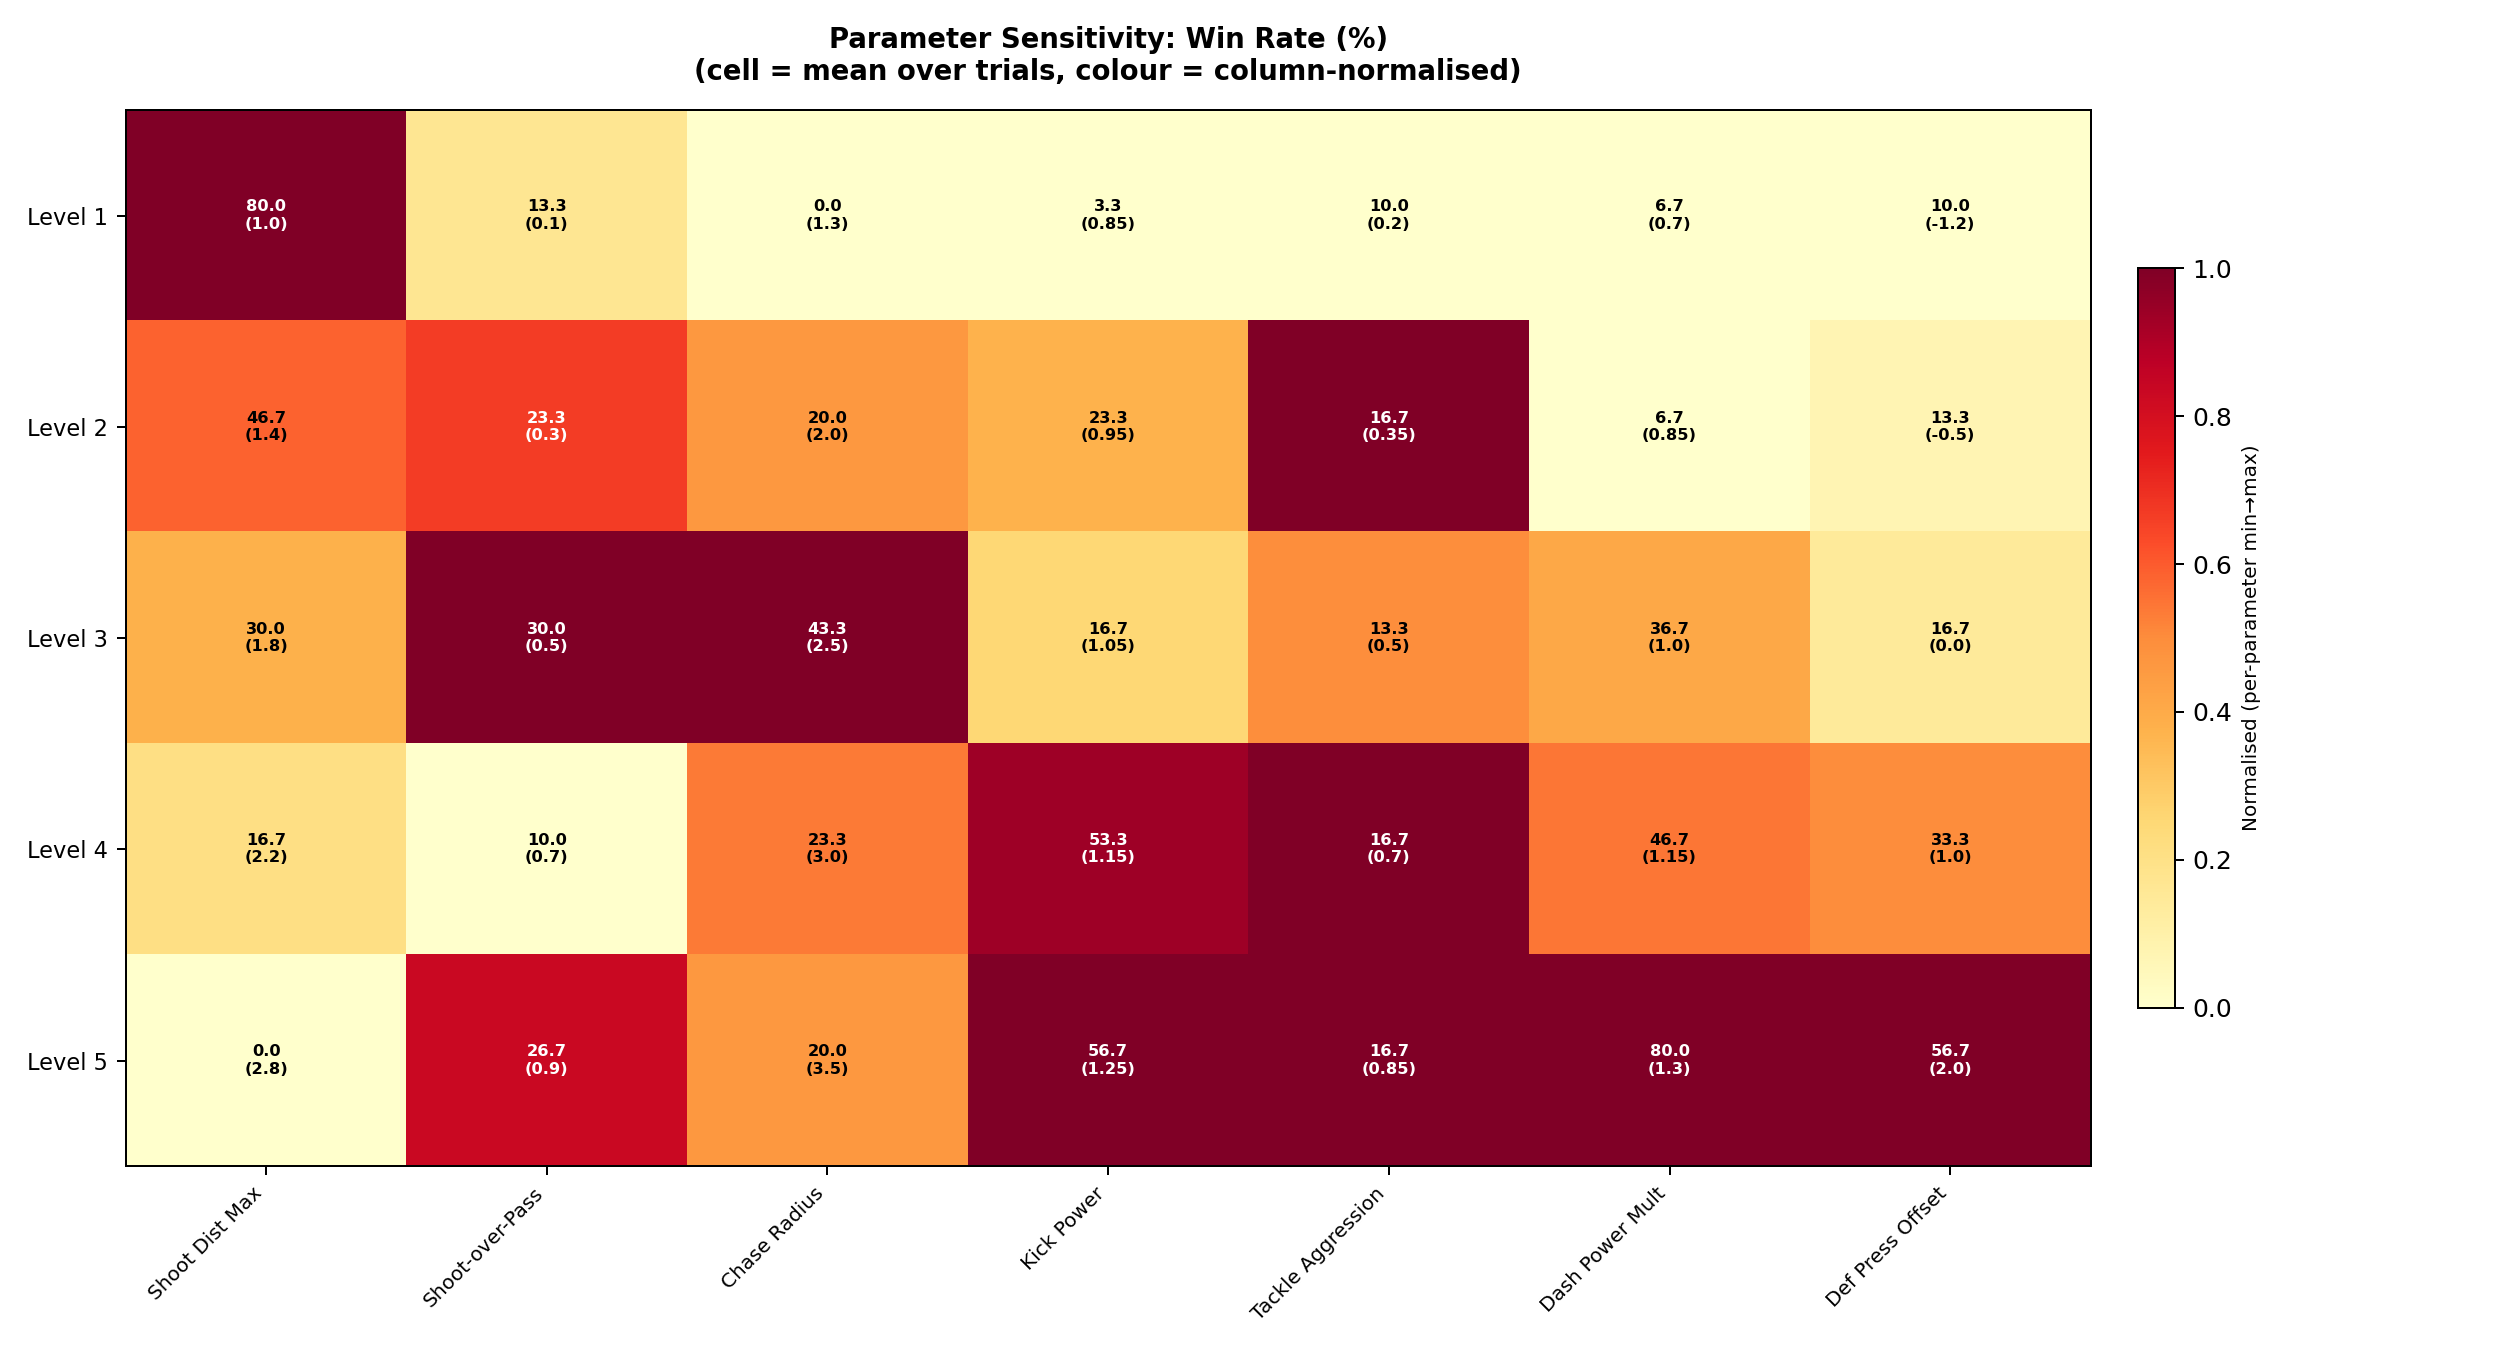
\includegraphics[width=0.85\textwidth]{heatmap_win_rate.png}
  \caption{Win Rate (\%) across all 7 parameters at 5 sweep levels.
    Darker shading indicates a higher win rate relative to the
    parameter's tested range.}
  \label{fig:winrate-heatmap}
\end{figure}

\begin{figure}[h]
  \centering
  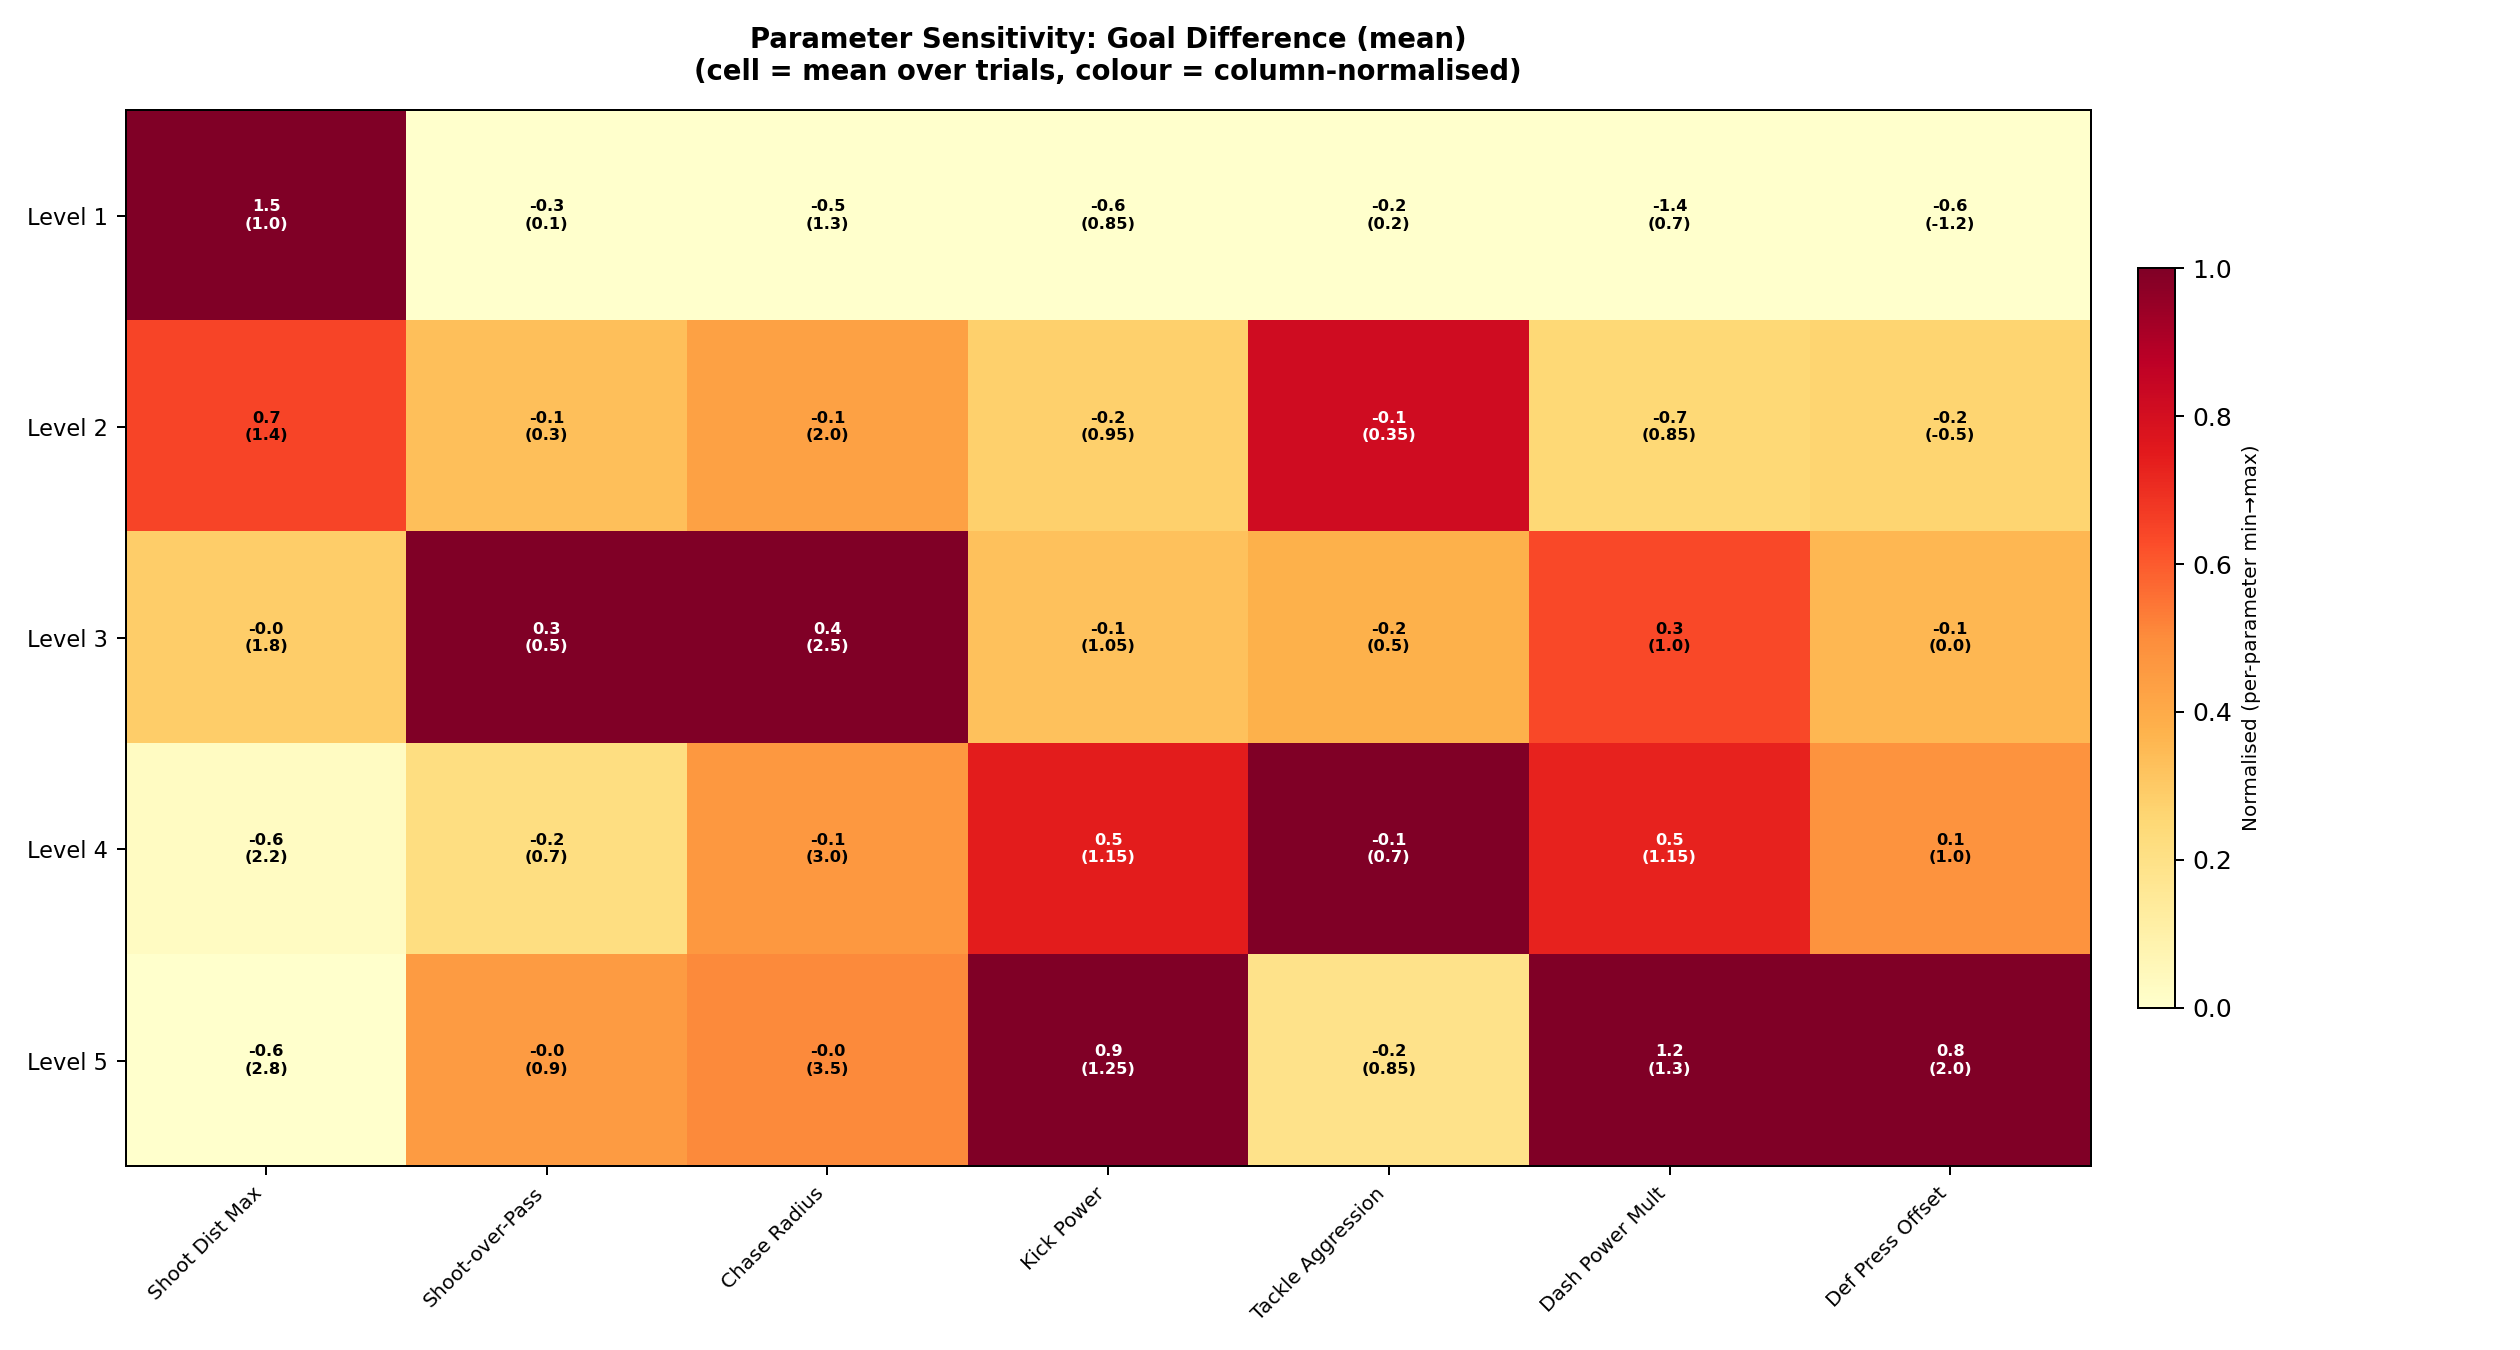
\includegraphics[width=0.85\textwidth]{heatmap_goal_difference.png}
  \caption{Average Goal Difference across all 7 parameters at 5 sweep
    levels. Positive values indicate a net scoring advantage for the
    experimental (Blue) team.}
  \label{fig:goaldiff-heatmap}
\end{figure}

This points to an important conclusion: regardless of how well the FSM
logic is designed, if the robot lacks the physical capability to reach the
ball before the opponent, it will lose possession and, with it, control of
the match.


\subsection{Quantity vs.\ Quality: Analysing the Shots Metrics}

The spatial threshold parameters revealed a consistent pattern across the
sweep: taking more shots did not lead to more wins. The data showed an
inverse relationship between shot volume and win rate, which points to the
importance of shot quality over quantity.
Note that the shot counts reported below are cumulative per-step totals
across a 24\,000-step match; the seemingly high figures reflect the
frequency at which the FSM enters the \texttt{KICKING} state rather than
human-scale kicks.

\paragraph{Shooting Distance.}
The maximum shooting distance parameter made this pattern clearest
(Figure~\ref{fig:totalshots-heatmap}).
When the robot was allowed to shoot from long range (2.8\,m), it averaged
1\,658 total shots per match and 251 forward-directed shots.
The Win Rate was \textbf{0.0\%} with a Goal Difference of $-0.63$.
Most of these shots were low-probability attempts that went straight to the
goalkeeper or opposing defenders, giving up possession without generating
goals.

Restricting the shooting trigger to within 1.0\,m of the goal reduced total
shots to 1\,611 per match and shots on target to just 126.
Despite the lower shot count, the Win Rate rose to \textbf{80.0\%} with a
maximum Goal Difference of $+1.47$.
Forcing the robot to wait for a closer position before shooting produced
better conversion and fewer wasted possessions.

\paragraph{Shots on Target Analysis.}
The shots on target heatmap (Figure~\ref{fig:sot-heatmap}) supports this
further.
At 2.8\,m shooting distance, the team registered 251 shots on target and
won 0\% of matches.
At 1.0\,m, only 126 shots on target were recorded, yet the team won 80\%.
This suggests that shots on target, as a metric, captures kicks where the
ball velocity is directed toward the opponent goal but the shot is still
easily saved.
What matters more is where the shot is taken from, not how many are aimed
in the right direction.

\paragraph{Shoot-Over-Pass Bias.}
The shoot-over-pass bias parameter pointed in the same direction.
Setting the bias to 0.1, which heavily favours passing, produced a positive
territory gain of $+12.4$, reflecting better spatial control of the pitch.
The raw win rate was modest at 13.3\% in isolation, but this is expected
when a single parameter is varied while the others remain at baseline.
The contribution of a disciplined passing approach becomes more significant
when combined with the other optimised parameters.

The full shot volume and shots on target heatmaps are included in
Appendix~\ref{app:heatmaps} (Figures~\ref{fig:totalshots-heatmap}
and~\ref{fig:sot-heatmap}).

\subsection{Territorial and Defensive Analysis}

The sweep also revealed patterns in how spatial parameters affected pitch
control.

\paragraph{Defensive Press Offset.}
This parameter controlled how far forward the defensive line sat when
without possession.
At the deepest setting ($-1.2$\,m), the team conceded territory (territory
gain of $-26.1$) and won only 10.0\% of matches.
At the most aggressive forward press ($+2.0$\,m), territory gain rose to
$+55.6$ and possession climbed to 73.0\%, producing a 56.7\% Win Rate.
However, $+1.0$\,m was selected as the final value (discussed in
Section~4.3.1) as a practical balance between pressing and defensive
exposure.

\paragraph{Chase Radius.}
The chase radius determined how far a field player would run to contest the
ball.
At the most restrictive setting (1.3\,m), the robots rarely engaged in
contested situations, yielding a 0.0\% Win Rate.
The best result occurred at 2.5\,m (43.3\% Win Rate, $+0.43$ Goal
Difference). Beyond this, over-extension caused formation problems; at
3.0\,m, the Win Rate dropped to 23.3\% with a territory deficit of $-23.2$.

\paragraph{Tackle Aggression.}
This parameter had the flattest response of all 7 variables, with win rates
ranging from 10.0\% (at 0.2) to 16.7\% (shared across three levels: 0.35,
0.7, and 0.85).
Its individual contribution was small, but its role becomes more relevant
when combined with high dash power and forward pressing, as discussed in
Section~4.3.2.

Territory gain and possession heatmaps across all tested parameter levels
are included in Appendix~\ref{app:heatmaps}
(Figures~\ref{fig:territory-heatmap} and~\ref{fig:possession-heatmap}).

\subsection{Limitations of the Sweep Methodology}

The 1\,050-match sweep provides useful empirical evidence, but several
limitations should be noted.

First, the OFAT approach tests each parameter in isolation, which means
interaction effects between parameters are not captured.
For example, the combined effect of high kick power and close shooting
distance may differ from what would be predicted by looking at each
independently.
A full factorial design would require $5^{7} = 78\,125$ parameter
combinations at 30 trials each, totalling over 2.3 million matches. This
was not feasible within the project timeline.
Alternative methods such as fractional factorial designs or Taguchi
orthogonal arrays could have captured key interaction effects in
substantially fewer runs~\cite{montgomery2017}.
OFAT was chosen for this study because it provides a clear, isolated
baseline response for each parameter, which was the primary objective
before any deeper integration analysis.

Second, a simulation-to-reality gap exists.
The Webots physics engine~\cite{webots2024} approximates real-world
friction, collision dynamics, and motor response, but cannot perfectly
replicate the behaviour of NAO6 hardware.
Parameters that appear optimal in simulation, particularly extreme dash
power values, may cause motor overheating or joint wear on the physical
platform.
This is why more conservative values were chosen for some parameters in the
Master List (Section~4.3.1).

Third, tackle aggression produced an essentially flat response in isolation.
Its inclusion in the final Master List at 0.7 is justified by a compound
effect: with dash power set to $1.3\times$, the robot arrives at tackle
situations faster, so a high aggression threshold ensures it capitalises on
that speed to win the ball rather than backing off.
However, this interaction was not formally quantified, and the individual
contribution of tackle aggression cannot be reliably isolated from this
sweep alone.

% -----------------------------------------------------------
\section{Behavioural Tactical Optimisation Results}

\subsection{Synthesis of the Optimal ``Master List''}

After analysing the 1\,050 asymmetric matches, an optimal parameter set was
compiled into a ``Master List.''
For each parameter, the value producing the highest win rate was the primary
candidate.
Where multiple levels produced similar win rates, secondary metrics
including goal difference, territory gain, and possession were used to
break the tie.
Hardware considerations, particularly the risk of motor wear and overheating
on physical RoboCup platforms~\cite{robocup2024}, also informed some final
selections.

It is worth noting that the selected kick power of $1.25\times$ exceeds the
value used in the codebase's built-in \texttt{AGGRESSIVE} preset
($1.15\times$). This value was retained for the simulation sweep because
the physics engine tolerates it without penalty, but for physical deployment
on a NAO6, the kick power would likely need to be reduced to stay within
the actuator's safe operating range.

\begin{table}[h]
  \centering
  \caption{The Optimal Behavioural Master List}
  \label{tab:master-list}
  \small
  \begin{tabular}{p{2.8cm} p{2.0cm} p{2.5cm} p{1.8cm} p{4.5cm}}
    \toprule
    \textbf{Parameter} & \textbf{Tested Range} & \textbf{Peak WR Value}
      & \textbf{Optimal} & \textbf{Justification} \\
    \midrule
    Shoot Distance Max & 1.0--2.8\,m & 1.0\,m (80.0\%) & \textbf{1.0\,m}
      & Clear peak; clinical shot philosophy \\
    Dash Power Multiplier & $0.7\times$--$1.3\times$ & $1.3\times$ (80.0\%)
      & $\mathbf{1.3\times}$
      & Clear peak; maximum mobility \\
    Kick Power Multiplier & $0.85\times$--$1.25\times$
      & $1.25\times$ (56.7\%)
      & $\mathbf{1.25\times}$
      & Clear peak; exceeds AGGRESSIVE preset, simulation-only \\
    Defensive Press Offset & $-1.2$--$+2.0$\,m & $+2.0$\,m (56.7\%)
      & $\mathbf{+1.0\,m}$
      & $+2.0$\,m risks counter-attack exposure; $+1.0$\,m provides
        33.3\% WR with balanced risk \\
    Chase Radius & 1.3--3.5\,m & 2.5\,m (43.3\%) & \textbf{2.5\,m}
      & Clear peak; beyond this, formation collapses \\
    Tackle Aggression & 0.2--0.85 & 0.7 (16.7\%) & \textbf{0.7}
      & Flat curve; 0.7 gives best goal difference ($-0.07$) among tied
        levels \\
    Shoot-Over-Pass Bias & 0.1--0.9 & 0.5 (30.0\%) & \textbf{0.1}
      & Selected for territory gain ($+12.4$) and passing discipline;
        compounds with close shooting distance \\
    \bottomrule
  \end{tabular}
\end{table}

\subsection{Synergistic Geometry and Behavioural Integration}

Each of these optimal values improves a specific aspect of play. When
combined, they produce a coherent strategy that is more effective than any
single parameter change in isolation.

An expanded chase radius (2.5\,m) combined with a forward defensive press
offset ($+1.0$\,m) pushes the robot higher up the pitch and into more
contested situations in the opponent's half.
When possession is won through tackles (at the 0.7 aggression threshold),
the strict 1.0\,m shooting distance means the robot carries the ball close
to goal before striking, which converts turnovers into high-quality
chances.
The low shoot-over-pass bias (0.1) means the robot circulates the ball
until the geometric conditions for a close-range shot are met, rather than
attempting speculative long-range efforts.

This combined effect is visible in the territory gain and possession
heatmaps (Figures~\ref{fig:territory-heatmap}
and~\ref{fig:possession-heatmap}).
Parameters that independently push the robot forward, including high dash
power, a forward press offset, and an expanded chase radius, reinforce each
other to produce sustained pressure in the opponent's half.

Importantly, the underlying FSM logic was not changed.
The core transition logic from Section~3.9 remained unchanged throughout.
By updating the \texttt{BehaviorProfile} class with the optimised Master
List, the robot's physical output and spatial decision boundaries were
shifted toward a more aggressive and precise strategy without modifying any
of the behavioural code.

\subsection{Final Validation Statistics}

To validate the Master List as a complete set, a final stress test was
conducted.
The ``Optimised Balanced Team,'' using all 7 Master List parameters at
once, was tested against the unmodified \texttt{BASELINE} profile over
\textbf{100 matches}, each running the full 20-minute RoboCup-compliant
duration~\cite{robocup2024}. Aggregate win/draw/goal statistics are stored
in \texttt{evaluate\_optimal.json}; per-match breakdowns with full
MetricsCollector outputs were not retained for this run.

\begin{table}[h]
  \centering
  \caption{Final Validation Results (100 Matches)}
  \label{tab:validation}
  \begin{tabular}{lcc}
    \toprule
    \textbf{Metric} & \textbf{Optimised Team (Blue)}
      & \textbf{Baseline Team (Red)} \\
    \midrule
    Win Rate          & \textbf{99.0\%}  & 0.0\%   \\
    Draw Rate         & 1.0\%            & 1.0\%   \\
    Avg Goals / Match & \textbf{4.36}    & 0.07    \\
    Avg Goal Diff.    & \textbf{$+4.29$} & $-4.29$ \\
    \bottomrule
  \end{tabular}
\end{table}

The results confirm that the parameter set works as intended.
Over 100 matches, the Optimised team achieved a \textbf{99.0\% Win Rate}
with a 1.0\% Draw Rate; the Baseline team won none.

The tactical adjustments produced an average of \textbf{4.36 goals per
match}, while the pressing and spatial constraints held the opponent to an
average of \textbf{0.07 goals conceded}, giving an average Goal
Differential of $+4.29$.
The key observation here is that none of the decision-making logic was
rewritten. The improvement came entirely from tuning the behavioural
parameters, which shows how much of a system's performance can depend on
how its physical and spatial boundaries are set.

It should be noted that this validation tests the Master List specifically
against the passive \texttt{BASELINE} opponent.
A 99\% win rate does not guarantee equal dominance against differently
tuned opponents.
Future work should test the Master List against a suite of randomised or
aggressively parameterised profiles to confirm that the optimised values
are broadly robust rather than over-fitted to the baseline's passivity.


% ============================================================
%  5. TEAM PERFORMANCE ANALYSIS  (~2.0 pages)
% ============================================================
\chapter{Team Performance Analysis}

% -----------------------------------------------------------
\section{Team Organisation Tools}
% Author(s): [assign member] | Target: 1.0 page


% -----------------------------------------------------------
\section{Team Performance Metrics}


% ============================================================
%  6. CONCLUSIONS AND FURTHER WORK  (~3.5 pages)
% ============================================================
\chapter{Conclusions and Further Work}

% -----------------------------------------------------------
\section{Conclusions}
% Author(s): [assign member] | Target: 2.5 pages


% -----------------------------------------------------------
\section{Further Work}
% Author(s): [assign member] | Target: 1.0 page


% ============================================================
%  REFERENCES
% ============================================================
\newpage
\addcontentsline{toc}{chapter}{References}

\begin{thebibliography}{9}

\bibitem{nash1950}
J.~F. Nash, ``Equilibrium Points in N-Person Games,''
\textit{Proceedings of the National Academy of Sciences},
vol.~36, no.~1, pp.~48--49, 1950.

\bibitem{montgomery2017}
D.~C. Montgomery, \textit{Design and Analysis of Experiments},
9th~ed. Hoboken, NJ: John Wiley \& Sons, 2017.

\bibitem{czitrom1999}
V.~Czitrom, ``One-Factor-at-a-Time versus Designed Experiments,''
\textit{The American Statistician},
vol.~53, no.~2, pp.~126--131, 1999.

\bibitem{robocup2024}
RoboCup Federation, \textit{RoboCup Soccer Humanoid League Rules and Setup},
2024. [Online]. Available: \url{https://humanoid.robocup.org/materials/rules/}

\bibitem{nao6specs}
SoftBank Robotics, \textit{NAO6 Technical Specifications},
2023. [Online]. Available: \url{https://www.aldebaran.com/en/nao}

\bibitem{webots2024}
Cyberbotics Ltd., \textit{Webots User Guide: Physics Engine},
2024. [Online]. Available: \url{https://cyberbotics.com/doc/guide}

\end{thebibliography}

% ============================================================
%  APPENDICES
% ============================================================
\appendix

\chapter{Parameter Definitions and NAO6 Mappings}
\label{app:params}

\begin{table}[H]
  \centering
  \caption{Parameter Definitions and NAO6 Hardware Mapping}
  \label{tab:param-defs}
  \small
  \begin{tabular}{p{3.0cm} p{3.5cm} p{1.8cm} p{5.0cm}}
    \toprule
    \textbf{Parameter} & \textbf{Physical Meaning} & \textbf{Units}
      & \textbf{NAO6 Mapping} \\
    \midrule
    Dash Power Multiplier
      & Scales the robot's walking gait speed relative to baseline
      & Dimensionless scalar
      & Maps to NAO6 joint motor velocity limits; $1.0\times$ represents
        the default walking gait, while $1.3\times$ approaches the
        platform's maximum sustainable stride frequency \\[4pt]
    Kick Power
      & Scales the force applied to the ball during a kick action
      & Dimensionless scalar
      & Corresponds to the torque output of the NAO6's leg actuators
        during the kick motion primitive \\[4pt]
    Shoot Distance Max
      & Maximum distance from the goal at which the robot will attempt
        a shot
      & Metres (m)
      & Defines the spatial trigger zone; beyond this radius the FSM
        will not transition to the \texttt{SHOOT} state \\[4pt]
    Chase Radius
      & Maximum distance from the ball at which a field player will
        sprint to contest possession
      & Metres (m)
      & Determines the spatial engagement zone; robots outside this
        radius ignore the ball and maintain formation \\[4pt]
    Defensive Press Offset
      & Vertical displacement of the defensive formation relative to
        the home position
      & Metres (m)
      & Positive values push defenders forward; negative values drop
        them deeper toward their own goal \\[4pt]
    Tackle Aggression
      & Probability threshold for attempting a tackle when within range
        of an opponent with the ball
      & Dimensionless (0--1)
      & $0.0$ = never tackles; $1.0$ = always tackles when
        geometrically possible \\[4pt]
    Shoot-Over-Pass Bias
      & Weighting between shooting and passing when both options are
        geometrically available
      & Dimensionless (0--1)
      & $0.0$ = always pass; $1.0$ = always shoot \\
    \bottomrule
  \end{tabular}
\end{table}

\chapter{Supporting Heatmaps}
\label{app:heatmaps}

\begin{figure}[H]
  \centering
  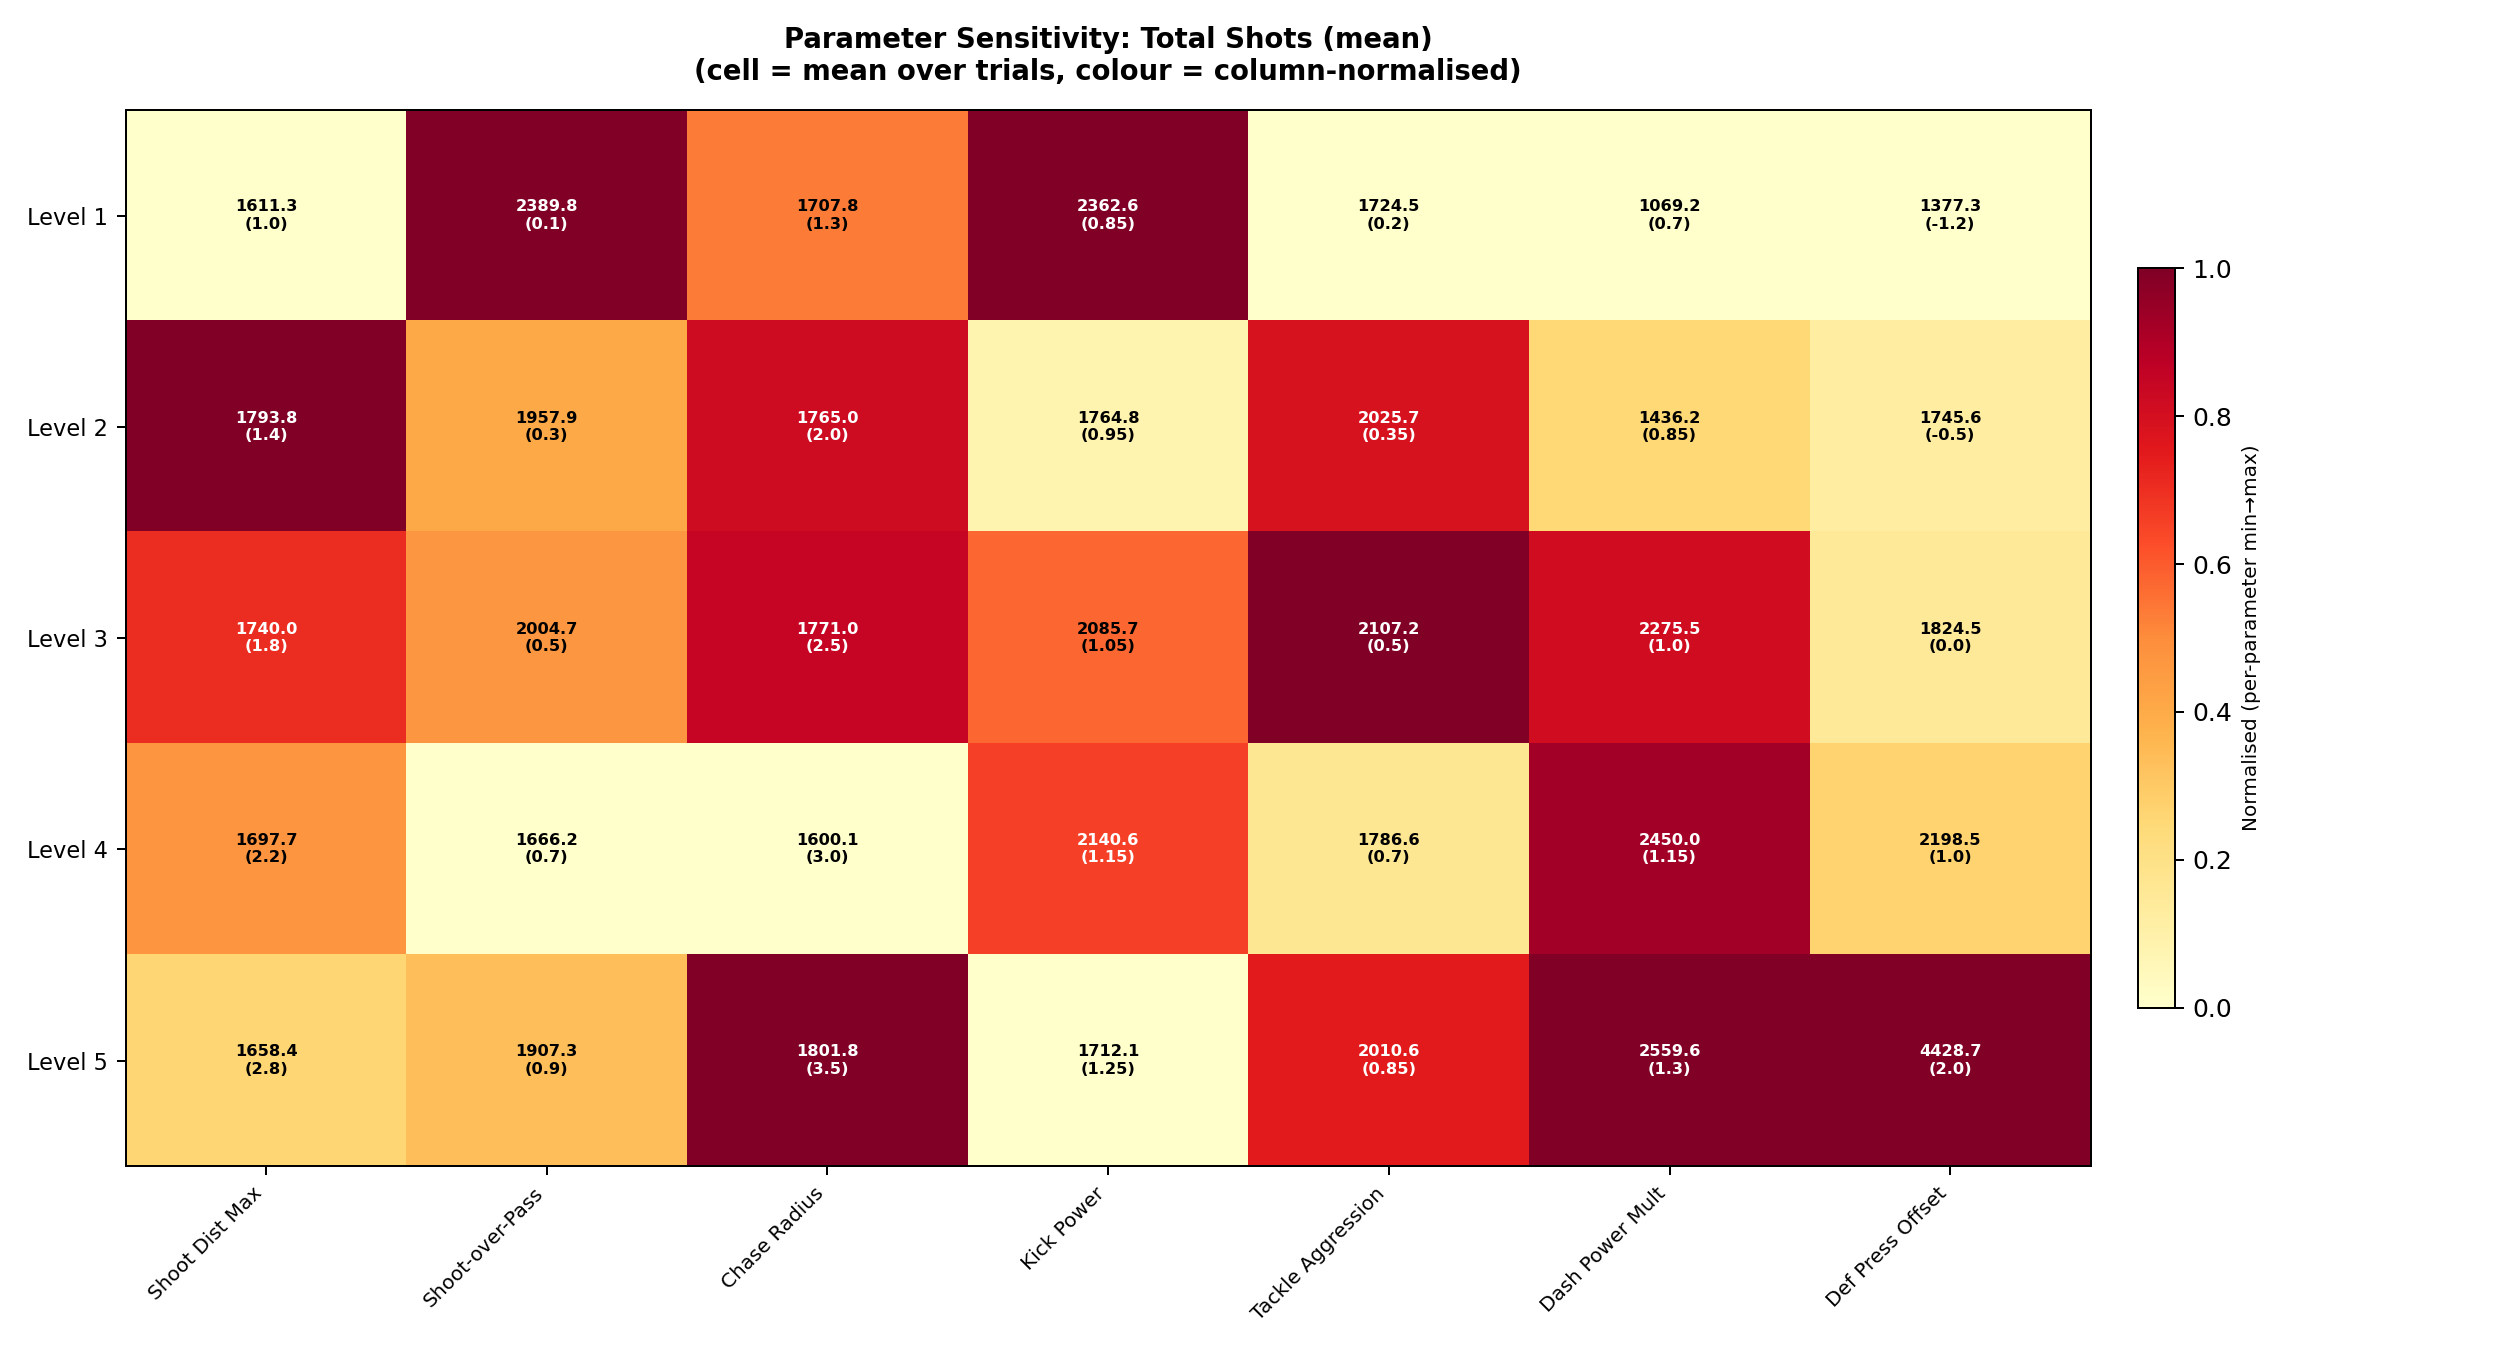
\includegraphics[width=0.85\textwidth]{heatmap_total_shots.png}
  \caption{Total shots per match across all 7 parameters at 5 sweep
    levels. High shot volume does not correlate with high win rate.}
  \label{fig:totalshots-heatmap}
\end{figure}

\begin{figure}[H]
  \centering
  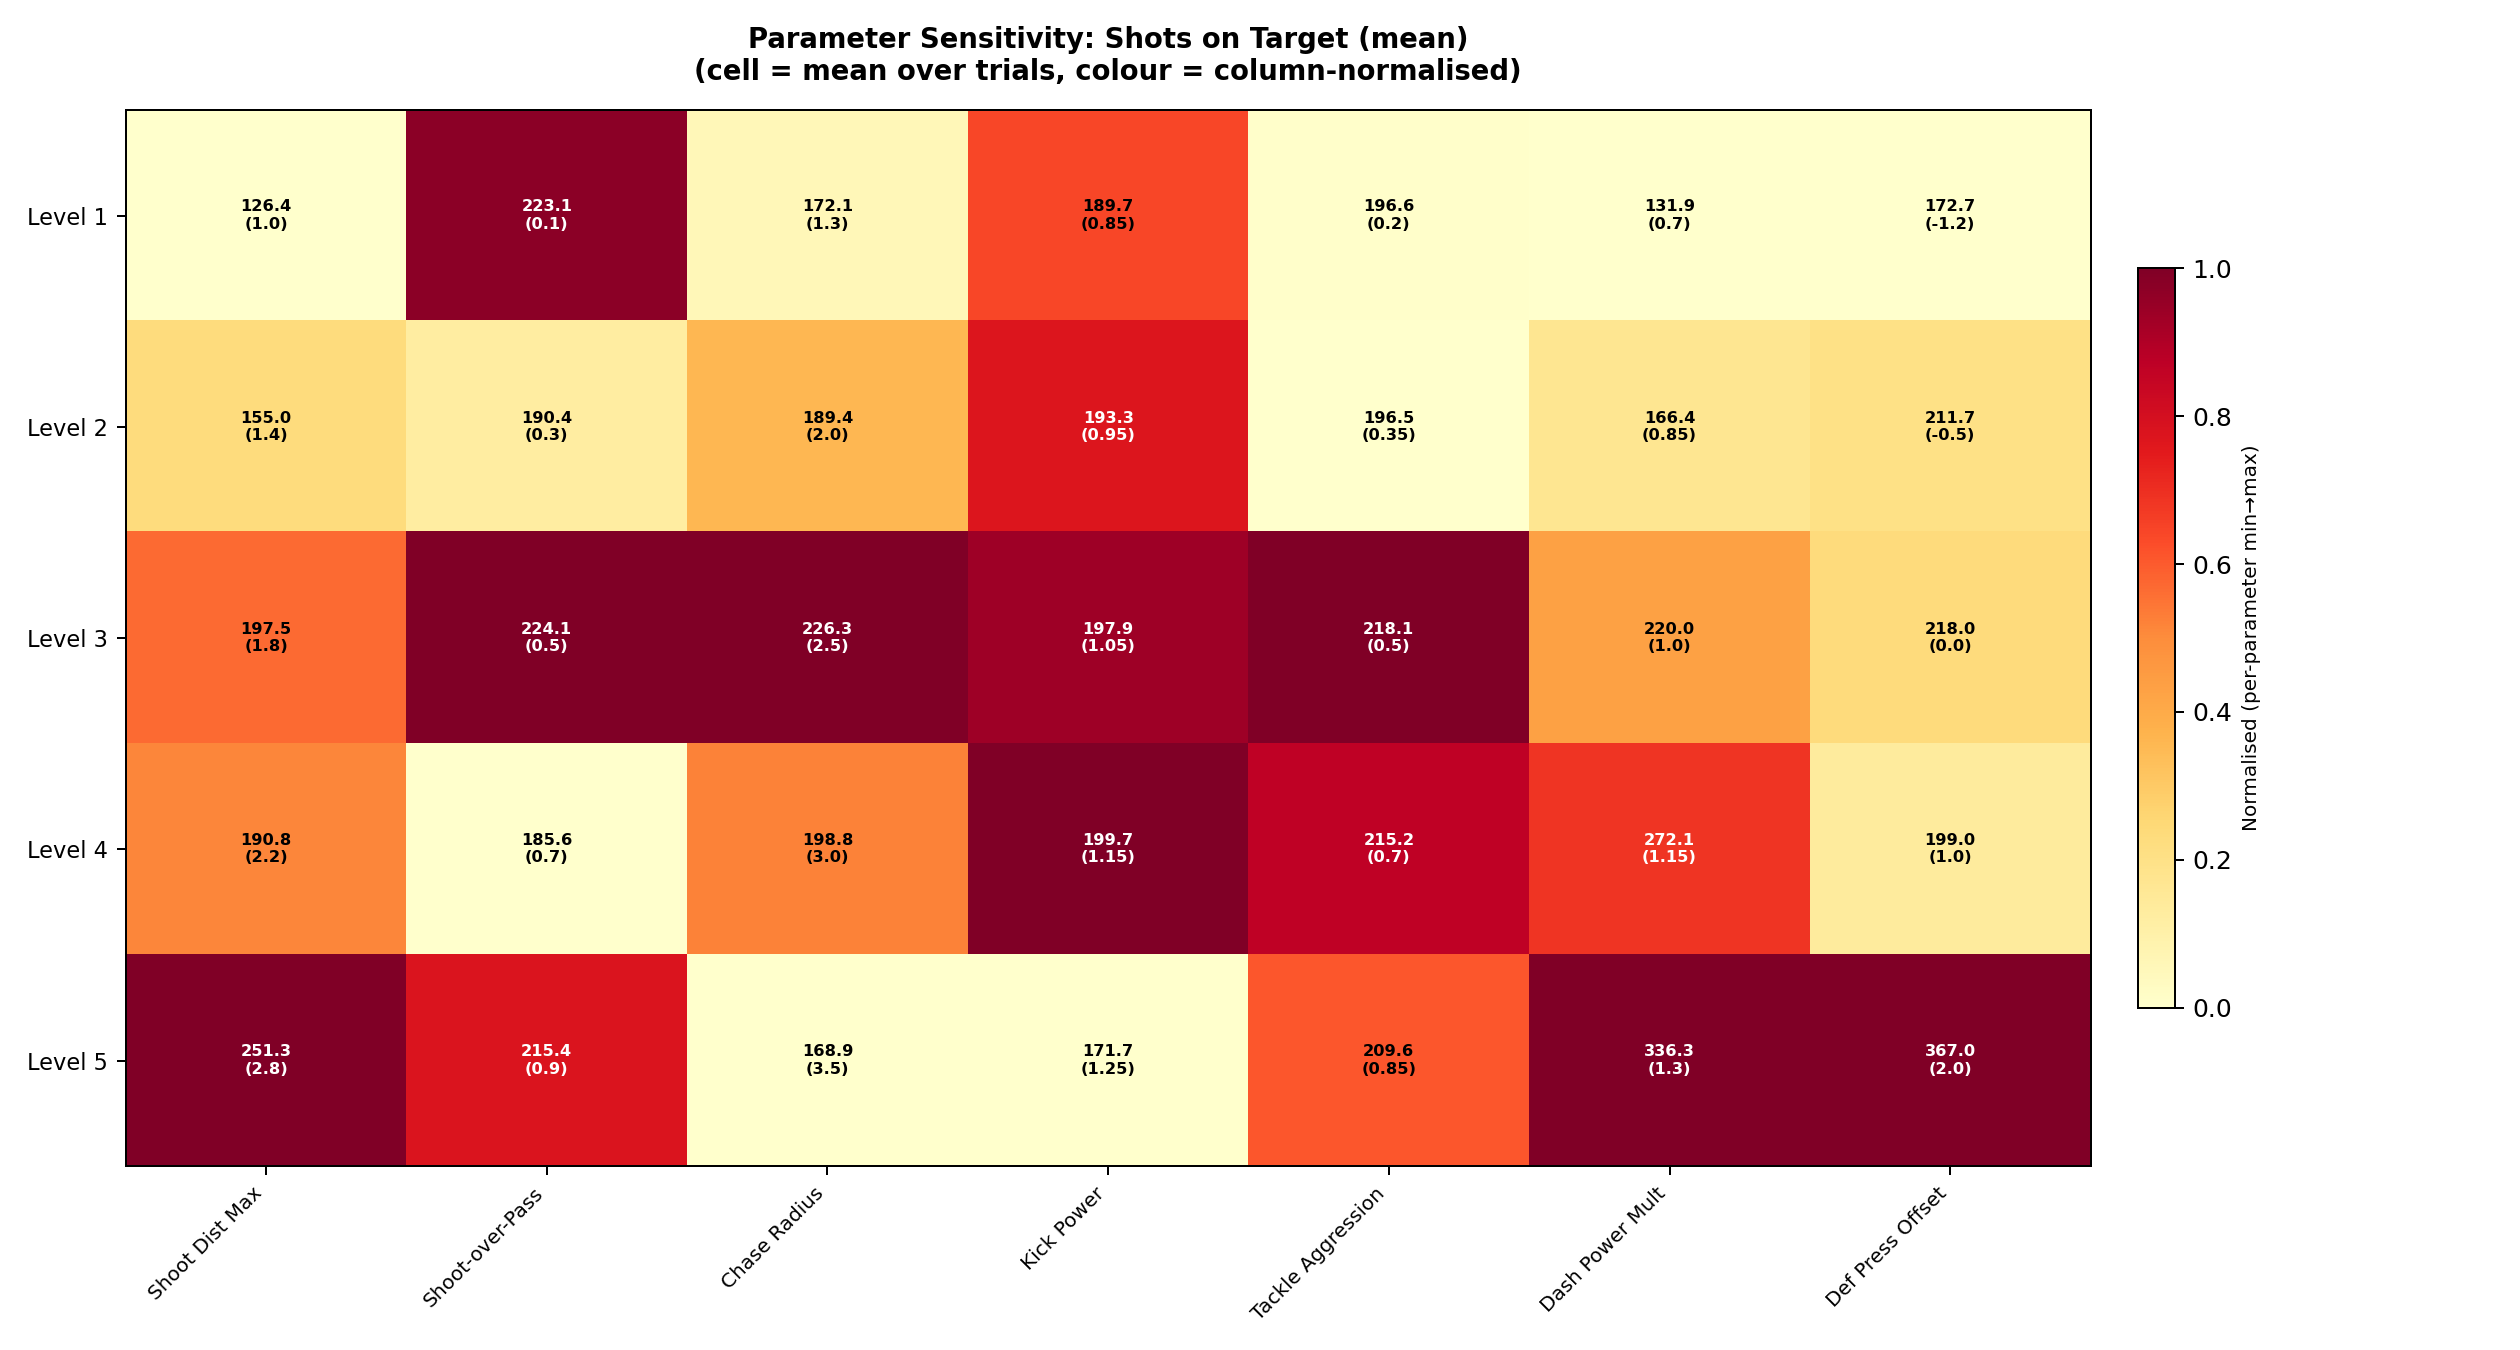
\includegraphics[width=0.85\textwidth]{heatmap_shots_on_target.png}
  \caption{Shots on target per match across all 7 parameters. High
    counts do not correlate with high win rates, indicating that shot
    proximity, not volume, drives conversion.}
  \label{fig:sot-heatmap}
\end{figure}

\begin{figure}[H]
  \centering
  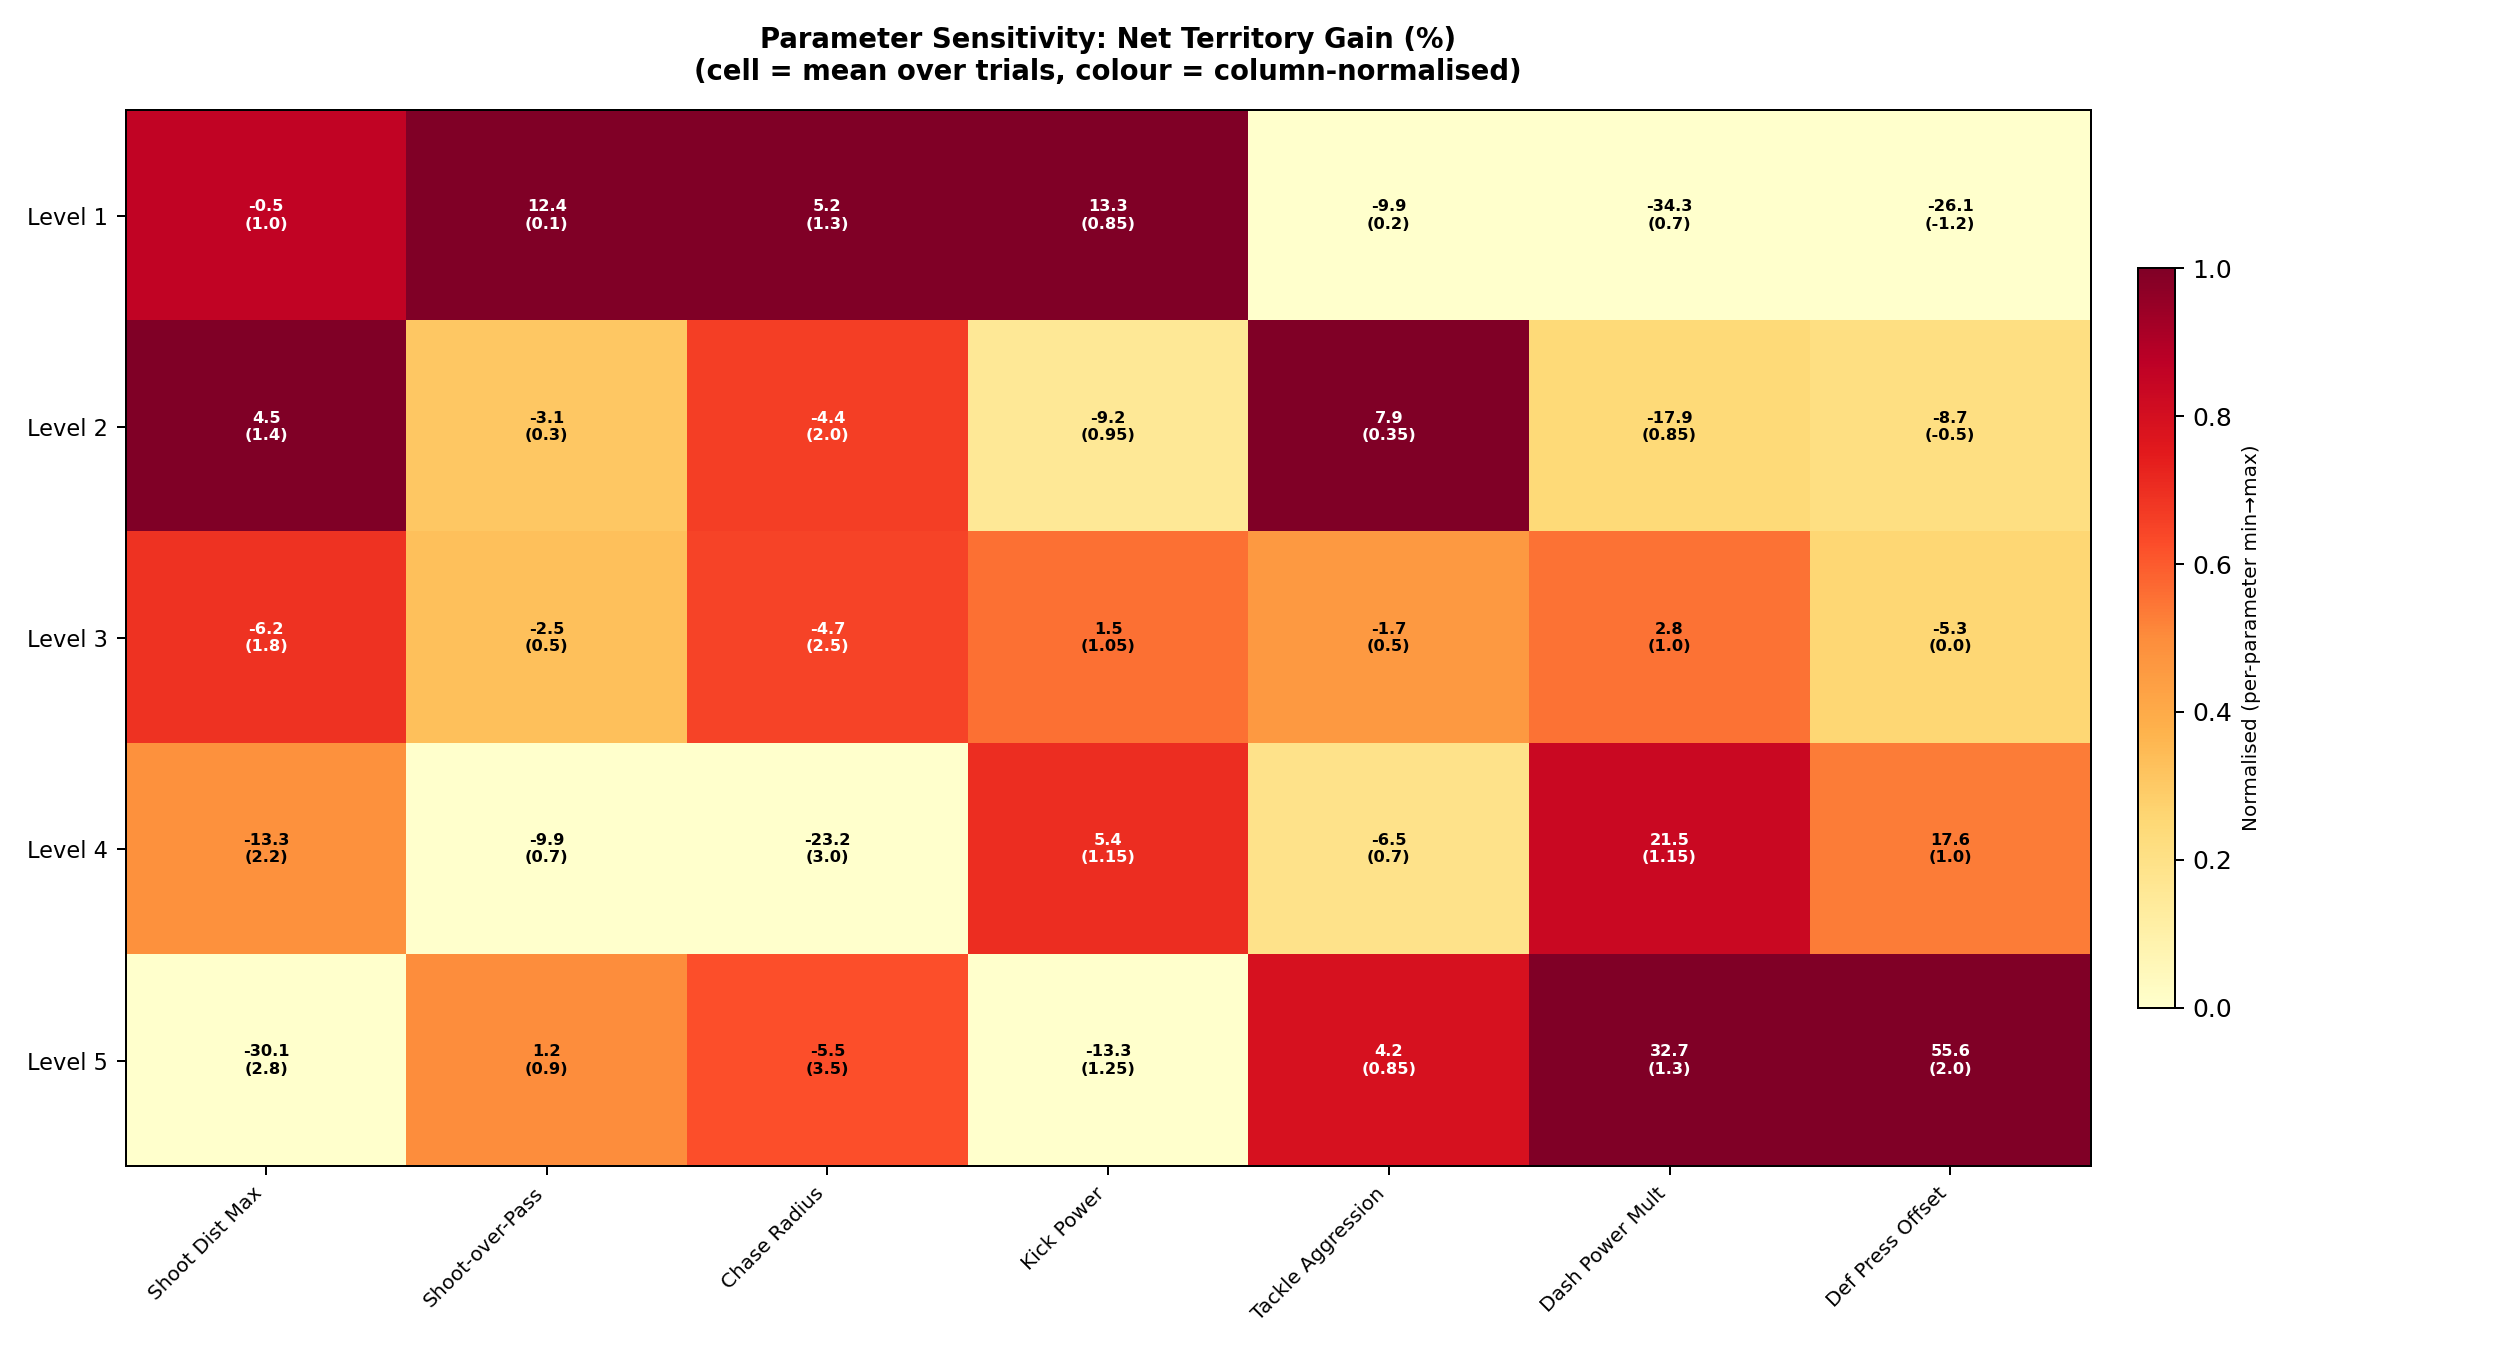
\includegraphics[width=0.85\textwidth]{heatmap_territory_gain.png}
  \caption{Net Territory Gain across all 7 parameters at 5 sweep
    levels. Positive values indicate territorial dominance for the
    experimental team.}
  \label{fig:territory-heatmap}
\end{figure}

\begin{figure}[H]
  \centering
  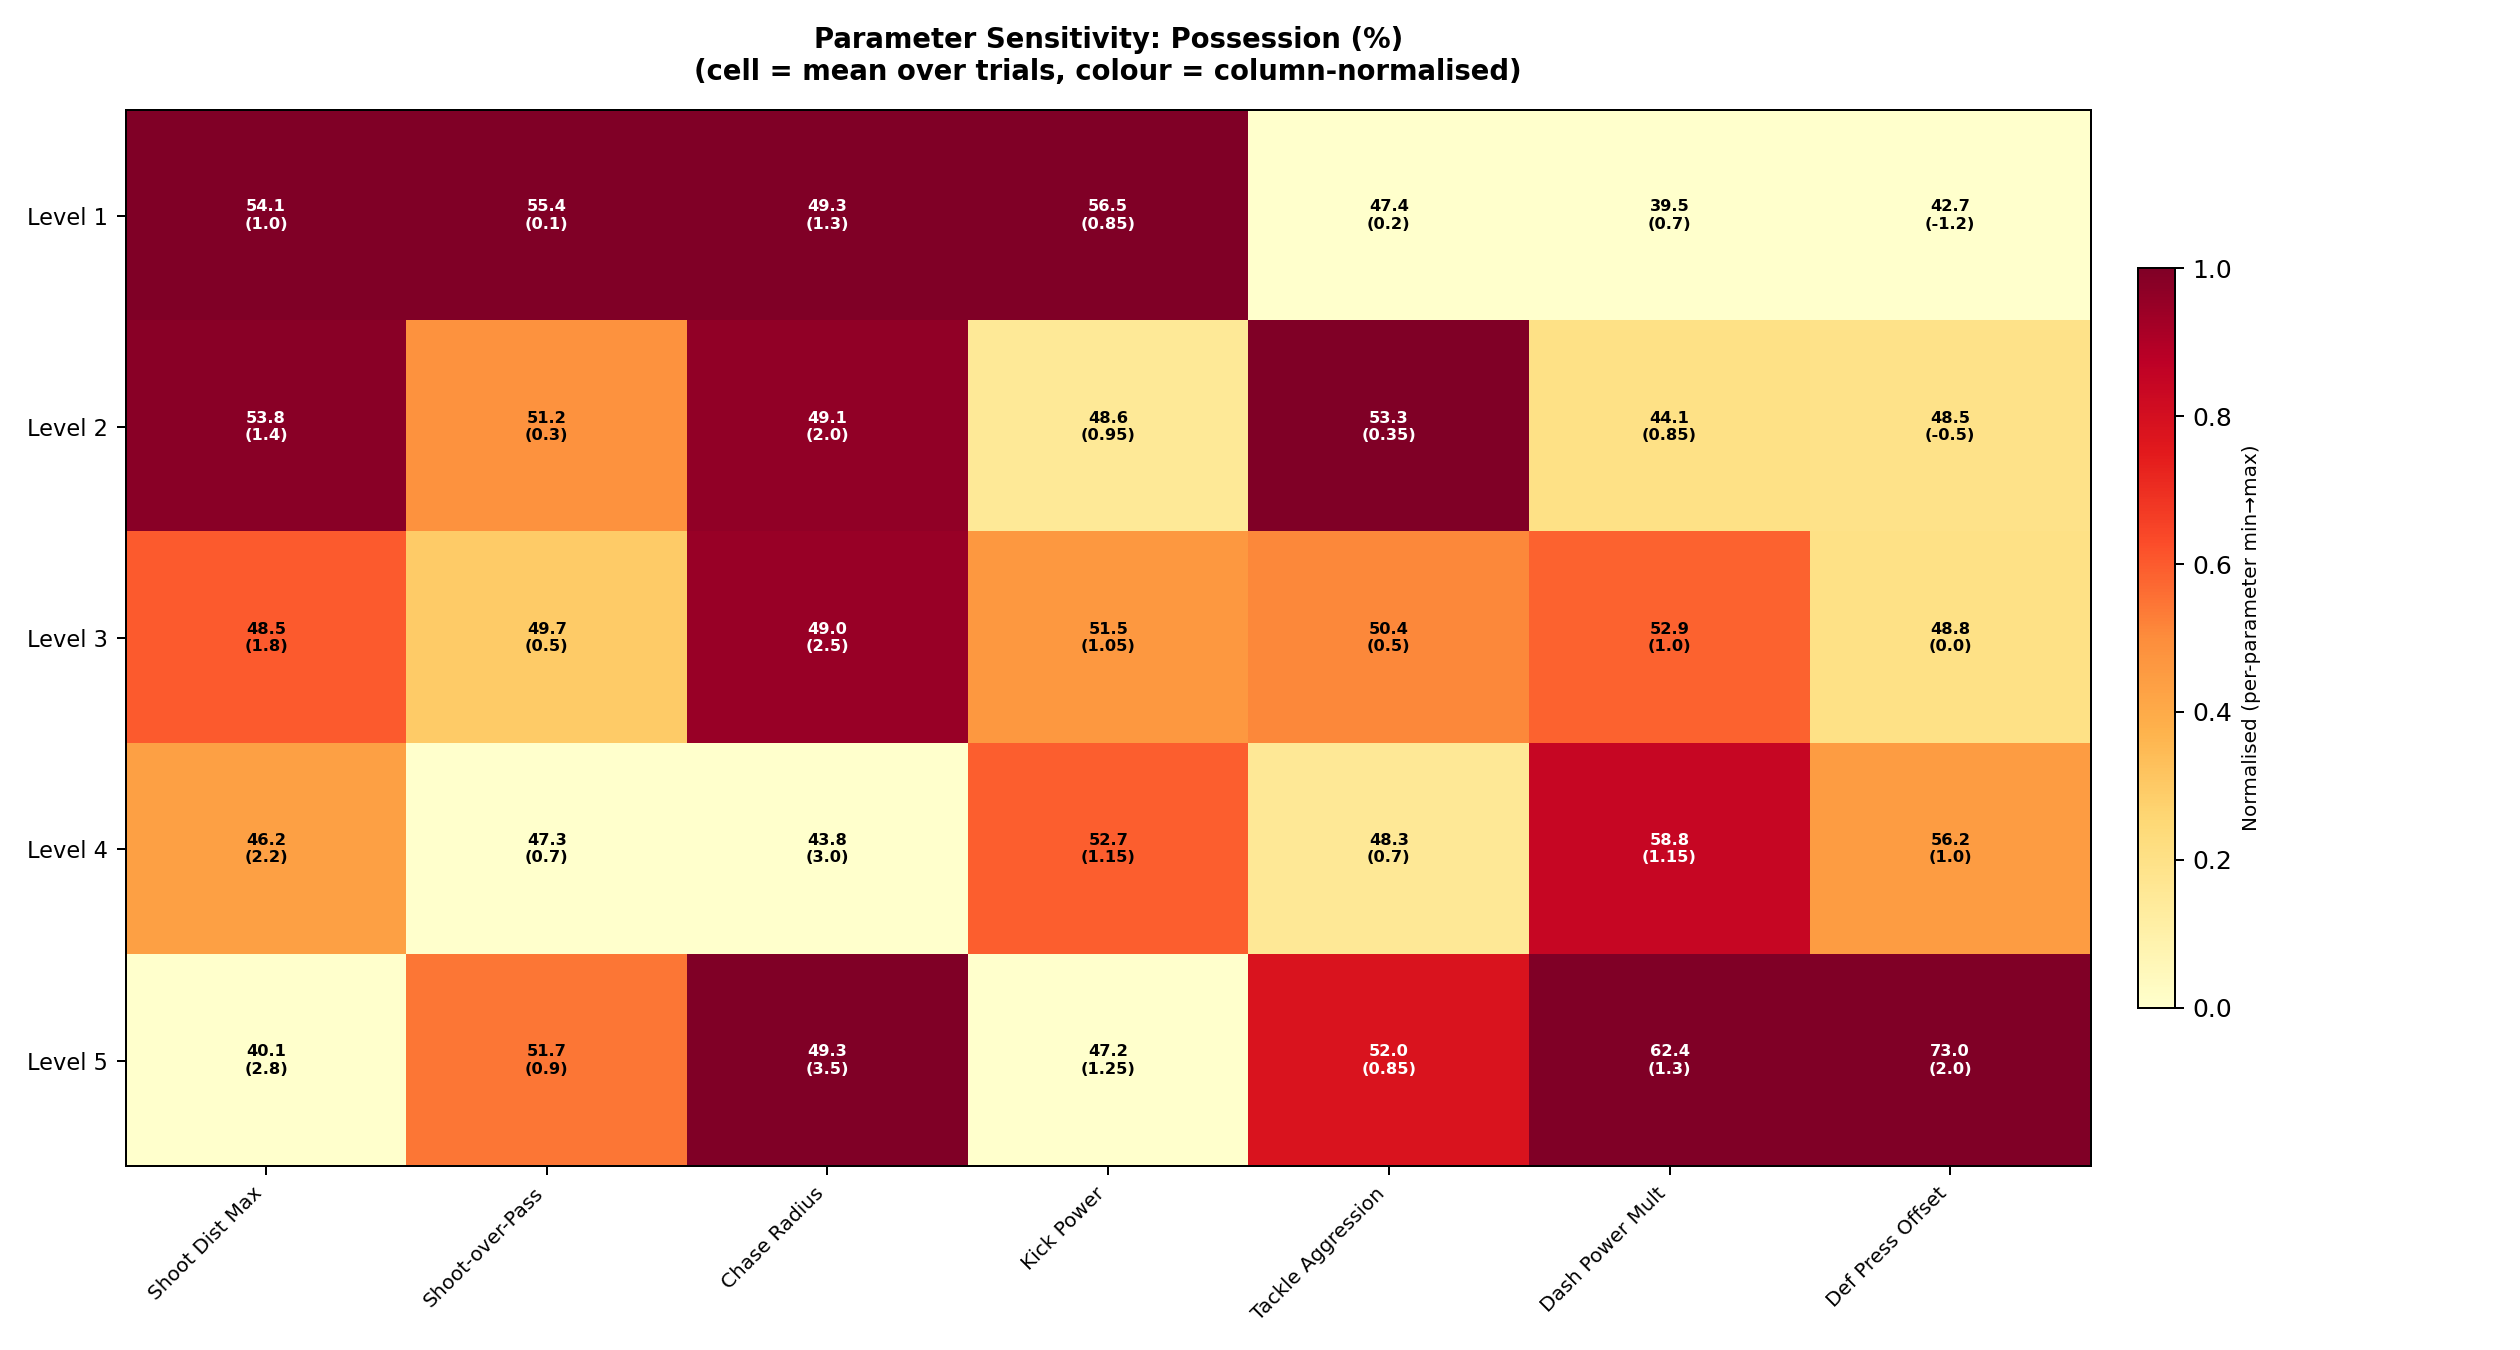
\includegraphics[width=0.85\textwidth]{heatmap_possession.png}
  \caption{Possession percentage across all 7 parameters at 5 sweep
    levels.}
  \label{fig:possession-heatmap}
\end{figure}

\end{document}
